\documentclass[hidelinks,12pt]{article}
\usepackage[left=0.25cm,top=1cm,right=0.25cm,bottom=1cm]{geometry}
%\usepackage[landscape]{geometry}
\textwidth = 20cm
\hoffset = -1cm
\usepackage[utf8]{inputenc}
\usepackage[spanish,es-tabla]{babel}
\usepackage[autostyle,spanish=mexican]{csquotes}
\usepackage[tbtags]{amsmath}
\usepackage{nccmath}
\usepackage{amsthm}
\usepackage{amssymb}
\usepackage{mathrsfs}
\usepackage{graphicx}
\usepackage{subfig}
\usepackage{standalone}
\usepackage[outdir=./Imagenes/]{epstopdf}
\usepackage{siunitx}
\usepackage{physics}
\usepackage{color}
\usepackage{float}
\usepackage{hyperref}
\usepackage{multicol}
%\usepackage{milista}
\usepackage{anyfontsize}
\usepackage{anysize}
%\usepackage{enumerate}
\usepackage[shortlabels]{enumitem}
\usepackage{capt-of}
\usepackage{bm}
\usepackage{relsize}
\usepackage{placeins}
\usepackage{empheq}
\usepackage{cancel}
\usepackage{wrapfig}
\usepackage[flushleft]{threeparttable}
\usepackage{makecell}
\usepackage{fancyhdr}
\usepackage{tikz}
\usepackage{bigints}
\usepackage{scalerel}
\usepackage{pgfplots}
\usepackage{pdflscape}
\pgfplotsset{compat=1.16}
\spanishdecimal{.}
\renewcommand{\baselinestretch}{1.5} 
\renewcommand\labelenumii{\theenumi.{\arabic{enumii}})}
\newcommand{\ptilde}[1]{\ensuremath{{#1}^{\prime}}}
\newcommand{\stilde}[1]{\ensuremath{{#1}^{\prime \prime}}}
\newcommand{\ttilde}[1]{\ensuremath{{#1}^{\prime \prime \prime}}}
\newcommand{\ntilde}[2]{\ensuremath{{#1}^{(#2)}}}

\newtheorem{defi}{{\it Definición}}[section]
\newtheorem{teo}{{\it Teorema}}[section]
\newtheorem{ejemplo}{{\it Ejemplo}}[section]
\newtheorem{propiedad}{{\it Propiedad}}[section]
\newtheorem{lema}{{\it Lema}}[section]
\newtheorem{cor}{Corolario}
\newtheorem{ejer}{Ejercicio}[section]

\newlist{milista}{enumerate}{2}
\setlist[milista,1]{label=\arabic*)}
\setlist[milista,2]{label=\arabic{milistai}.\arabic*)}
\newlength{\depthofsumsign}
\setlength{\depthofsumsign}{\depthof{$\sum$}}
\newcommand{\nsum}[1][1.4]{% only for \displaystyle
    \mathop{%
        \raisebox
            {-#1\depthofsumsign+1\depthofsumsign}
            {\scalebox
                {#1}
                {$\displaystyle\sum$}%
            }
    }
}
\def\scaleint#1{\vcenter{\hbox{\scaleto[3ex]{\displaystyle\int}{#1}}}}
\def\bs{\mkern-12mu}


\title{Ondas transversales en coordenadas cilíndricas \\[0.3em]  \large{Matemáticas Avanzadas de la Física}\vspace{-3ex}}
\author{M. en C. Gustavo Contreras Mayén}
\date{ }

\begin{document}
\vspace{-4cm}
\maketitle
\fontsize{14}{14}\selectfont
\tableofcontents
\newpage

\section{Marco de referencia.}

\subsection{Guías de ondas.}

Una guía de ondas es una estructura elaborada por conductores, dieléctricos, o una combinación de éstos, cuenta con una sección recta constante en una dirección que permite propagar o guiar ondas electromagnéticas ya sea en su interior, en sus proximidades o en ambas regiones.
\begin{figure}[H]
    \centering
    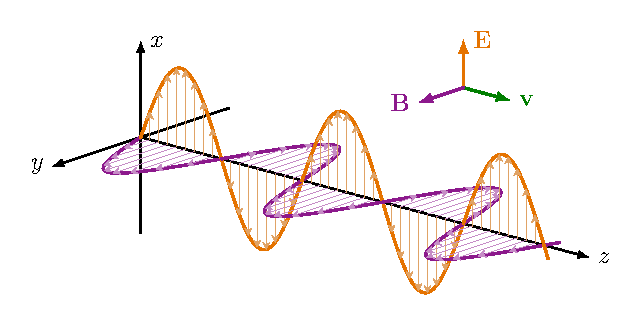
\includegraphics[scale=1]{Imagenes/Onda_Electromagnetica.eps}
    \caption{Onda electromagnética.}
\end{figure}
La geometría de la guía de onda queda determinada por la forma y frecuencia de las ondas que deben propagar, como se aprecia en la figura (\ref{fig:figura_01}):
\begin{figure}[H]
    \centering
    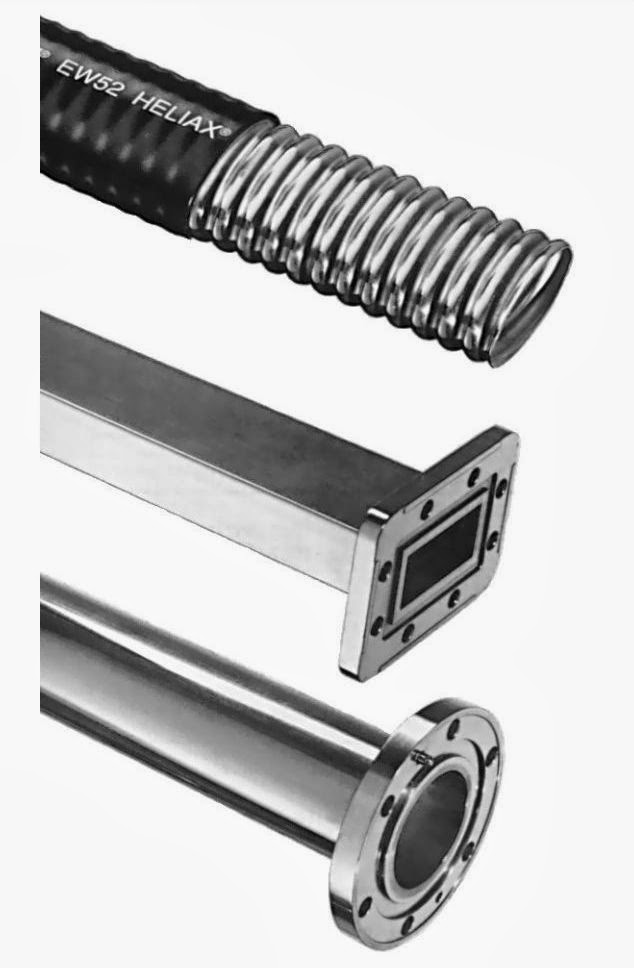
\includegraphics[scale=0.25]{Imagenes/Tubos_Guias_Onda.jpg}
    \caption{Tres tipos de guías de onda: elíptico, rectangular y circular.}
    \label{fig:figura_01}
\end{figure}

Las guías de onda son adecuadas para transmitir señales debido a su bajas pérdidas. Por ello, se usan en microondas, a pesar de su ancho de banda limitado y volumen, mayor que el de líneas impresas o coaxiales para la misma frecuencia. En la figura (\ref{fig:figura_02}) se muestra un esquema de una guía de onda de tipo coaxial.

\begin{figure}[H]
    \centering
    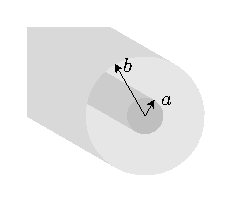
\includegraphics[scale=1.4]{Imagenes/Guia_Onda_Coaxial.eps}
    \caption{Esquema de una guía de onda coaxial con radio interno $a$ y radio externo $b$.}
    \label{fig:figura_02}
\end{figure}

Las ecuaciones generales que describen el comportamiento de los campos que se propagan en las guías de onda, son soluciones generales de las ecuaciones de Maxwell, como consideraciones debemos de tomar en cuenta que:
\begin{enumerate}
\item Las ondas se generan únicamente con señales senoidales.\item Las guías de onda son infinitamente largas.
\item La dirección de propagación de los campos está en la dirección $z$, según los ejes de coordenadas cartesianas o cilíndricas.
\end{enumerate}

Estas ecuaciones tienen soluciones múltiples, o modos. Los modos de propagación dependen de la longitud de onda, de la polarización y de las dimensiones de la guía. El \emph{modo longitudinal} de una guía de onda es un tipo particular de onda estacionaria formado por ondas confinadas en la cavidad.

\subsection{Modos de Propagación.}

Los modos transversales se clasifican en distintos tipos:
\begin{enumerate}[label=\roman*)]
\item Modo TE (Transversal eléctrico), la componente de $\vb{E}$ en la dirección de propagación es nula.
\item Modo TM (Transversal magnético), la componente de $\vb{B}$ en la dirección de propagación es nula.
\item Modos TEM (Transversal electromagnético), la componente tanto del $\vb{E}$ como de $\vb{B}$ en la dirección de propagación es nula.
\item Modos híbridos: son los que sí tienen componente en la dirección de propagación tanto en el campo eléctrico como en el de inducción magnética.
\end{enumerate}

\section{El Laplaciano de una función vectorial.}

El Laplaciano de un campo vectorial $\vb{V}$, que se expresa como $\laplacian{\vb{V}}$, se define como:
\begin{align*}
\laplacian{\vb{V}} = \grad{\div{\vb{V}}} - \curl{\curl{\vb{V}}}
\end{align*}

En problemas de guías de ondas circulares y resonadores de cavidades cilíndricas, el Laplaciano vectorial en coordenadas cilíndricas circulares es:
\begin{align*}
\laplacian{\va{V}} \Rightarrow \begin{cases}
\laplacian{V_{\rho}} = \laplacian{V_{\rho}} - \dfrac{1}{\rho} V_{\rho} - \dfrac{2}{\rho^{2}} \displaystyle \pdv{V_{\varphi}}{\varphi} \\[0.75em]
\laplacian{V_{\varphi}} = \laplacian{V_{\varphi}} - \dfrac{1}{\rho} V_{\varphi} - \dfrac{2}{\rho^{2}} \displaystyle \pdv{V_{\rho}}{\varphi} \\[0.75em]
\laplacian{V_{z}} = \laplacian{V_{z}}
\end{cases}
\end{align*}
En donde podemos notar que el Laplaciano de una función escalar es similar a la componente $z$ del Laplaciano de un campo vectorial.

\section{Enunciado del ejercicio.}

Una onda electromagnética transversal en una guía de onda coaxial tiene un campo eléctrico $\vb{E} = \vb{E} (\rho, \varphi) \, \exp(i [k z - \omega t])$ y un campo de inducción magnética $\vb{B} = \vb{B} (\rho, \varphi) \, \exp(i [k z - \omega t])$. Como la onda es transversal, ni $\vb{E}$ ni $\vb{B}$ tiene componente $z$. Los dos campos satisfacen la ecuación de Laplace vectorial:
\begin{align*}
\laplacian{\vb{E} (\rho, \varphi)} &= 0 \\[0.5em]
\laplacian{\vb{B} (\rho, \varphi)} &= 0
\end{align*}

\begin{enumerate}[label=\alph*)]
\item Demuestra que:
\begin{align*}
\vb{E} &= \vu{\bm{\rho}} \, \bigg( \dfrac{a}{\rho} \bigg) E_{0} \, \exp(i [k z - \omega t]) \\[0.5em]
\vb{B} &= \vu{\bm{\varphi}} \, \bigg( \dfrac{a}{\rho} \bigg) B_{0} \, \exp(i [k z - \omega t])
\end{align*}
son soluciones. Considera que $a$ es el radio del conductor interno y $E_{0}$ y $B_{0}$ son amplitudes constantes.
\item Suponiendo que hay vacío dentro de la guía de onda, verifica que las ecuaciones de Maxwell se satisfacen con:
\begin{align*}
\dfrac{B_{0}}{E_{0}} = \dfrac{k}{\omega} = \mu_{0} \varepsilon_{0} \bigg( \dfrac{\omega}{k} \bigg) = \dfrac{1}{c}
\end{align*}
\end{enumerate}

\section{Solución.}

\noindent
\textbf{Inciso a):} Para $\vb{E} (\rho, \varphi)$, la ecuación relevante es la que contiene la componente $\rho$ del vector Laplaciano, ya que las otras componentes se anulan:
\begin{align*}
\laplacian{E} &= \laplacian{E_{\rho}} - \dfrac{1}{\rho^{2}} E_{\rho} = \\[0.5em]
&= \dfrac{1}{\rho} \pdv{\rho} \bigg( \rho \pdv{E_{\rho}}{\rho} \bigg) - \dfrac{1}{\rho^{2}} E_{\rho} = \\[0.5em]
&= \dfrac{1}{\rho} \pdv{\rho} \bigg( - \dfrac{a}{\rho} E_{0} \bigg) - \dfrac{a}{\rho^{3}} E_{0} = \\[0.5em]
&= \dfrac{a}{\rho^{3}} E_{0} - \dfrac{a}{\rho^{3}} E_{0} = \\[0.5em]
&= 0
\end{align*}

Para $\vb{B} (\rho, \varphi)$, la ecuación relevante es la que contiene la componente $\varphi$ del vector Laplaciano:
\begin{align*}
\laplacian{\vb{B}} &= \laplacian{B_{\varphi}} - \dfrac{1}{\rho^{2}} B_{\varphi} = \\[0.5em]
&= \dfrac{1}{\rho^{2}} B_{\varphi} - \dfrac{1}{\rho^{2}} B_{\varphi} = \\[0.5em]
&= 0
\end{align*}

\noindent
\textbf{Inciso b):} Para verificar que las soluciones satisfacen las ecuaciones de Maxwell, debemos de expresar tanto la divergencia como el rotacional de $\vb{E}$ y $\vb{B}$.

\noindent
Para el campo eléctrico $\vb{E}$:
\begin{align*}
0 &= \div{\vb{E}} = \dfrac{1}{\rho} \pdv{\rho} \bigg( \rho E_{\rho} \bigg) + \dfrac{1}{\rho} \pdv{E_{\rho}}{\varphi} + \pdv{E_{z}}{z} = \\[0.5em]
&= \dfrac{1}{\rho} \pdv{\rho} \bigg( a E_{0} \bigg) = \\[0.5em]
&= 0
\end{align*}

\noindent
Para el campo de inducción magnética $\vb{B}$:
\begin{align*}
0 &= \div{\vb{B}} = \dfrac{1}{\rho} \pdv{\rho} \bigg( \rho B_{\rho} \bigg) + \dfrac{1}{\rho} \pdv{B_{\rho}}{\varphi} + \pdv{B_{z}}{z} = \\[0.5em]
&= \dfrac{1}{\rho} \pdv{\rho} \bigg( a B_{0}\bigg) = \\[0.5em]
&= 0
\end{align*}

\noindent
Para el rotacional de $\vb{E}$:
\begin{align*}
0 &= \curl{\vb{E}} + \pdv{\vb{B}}{t} = \\[0.5em]
&= \dfrac{1}{\rho} \mqty|
\vu{\bm{\rho}} & \rho \, \vu{\bm{\varphi}} & \vu{z} \\[0.5em]
\displaystyle \pdv{\rho} & \displaystyle  \pdv{\varphi} & \displaystyle \pdv{z} \\[0.5em]
E_{\rho} & E_{\varphi} & E_{z} | + \pdv{\vb{B}}{t} = \\[0.5em]
&= \dfrac{1}{\rho} \bigg[ - \vu{\bm{\varphi}} \, i \, k \, a \, E_{0} \, \exp(i [k z - \omega t]) - 0 \bigg] + \\[0.5em]
&+ \vb{\bm{\varphi}} \, (- i \omega) \dfrac{a}{\rho} \, B_{0} \, \exp(i [k z - \omega t]) = \\[0.5em]
&= \vb{\bm{\varphi}} \, \dfrac{i \, a}{\rho} \, \exp(i [k z - \omega t]) \bigg[ k \, E_{0} - \omega \, B_{0} \bigg]
\end{align*}
para que se cumpla la igualdad, se debe de cumplir:
\begin{align*}
k \, E_{0} - \omega \, B_{0} &= 0 \\[0.5em]
\Rightarrow \hspace{0.2cm} k \, E_{0} &= \omega \, B_{0} \\[0.5em]
\Rightarrow \hspace{0.2cm} \dfrac{B_{0}}{E_{0}} &= \dfrac{k}{\omega}
\end{align*}
que es la condición que se señaló en el enunciado.

\noindent
Para el campo de inducción magnética $\vb{B}$:
\begin{align*}
0 &= \curl{\vb{B}} - \mu_{0} \, \varepsilon_{0} \, \pdv{\vb{E}}{t} = \\[0.5em]
&= \dfrac{1}{\rho} \mqty|
\vu{\bm{\rho}} & \rho \, \vu{\bm{\varphi}} & \vu{z} \\[0.5em]
\displaystyle \pdv{\rho} & \displaystyle  \pdv{\varphi} & \displaystyle \pdv{z} \\[0.5em]
B_{\rho} & B_{\varphi} & B_{z} | - \mu_{0} \, \varepsilon_{0} \, \pdv{\vb{E}{t}} = \\[0.5em]
&= \dfrac{1}{\rho} \bigg[ 0 - \vu{\bm{\rho}} \, i \, k \, a \, B_{0} \, \exp(i [k z - \omega t]) \bigg] + \\[0.5em]
&- \vu{\bm{\rho}} \, \mu_{0} \, \varepsilon_{0} (- i \, \omega) \dfrac{a}{\rho} E_{0} \, \exp(i [k z - \omega t]) = \\[0.5em]
&= \vu{\bm{\rho}} \, \dfrac{i \, a}{\rho} \, \exp(i [k z - \omega t]) \, \bigg( - k \, B_{0} + \mu_{0} \, \varphi_{0} \, E_{0} \bigg)
\end{align*}
para que se cumpla la igualdad, debe de ocurrir que:
\begin{align*}
- k \, B_{0} + \mu_{0} \, \varphi_{0} \, E_{0} &= 0 \\[0.5em]
\Rightarrow \hspace{0.3cm} k \, B_{0} = \mu_{0} \, \varphi_{0} \, E_{0} \\[0.5em]
\Rightarrow \hspace{0.3cm} \dfrac{B_{0}}{E_{0}} = \dfrac{\mu_{0} \, \varphi_{0} \, \omega}{k}
\end{align*}
tal como se indicó en el enunciado del ejercicio.
\end{document}